\documentclass[aspectratio=169,10pt]{beamer}

\usepackage{amsmath,amssymb}
\usepackage{graphicx}
\usepackage{caption}
\usepackage{biblatex}
\addbibresource{ref.bib}
\setbeamerfont{footnote}{size=\tiny}
\usetheme{CambridgeUS}
\usecolortheme{seahorse}
\usefonttheme{serif}
\pgfdeclareimage[height=0.5cm]{university-logo}{logo.png}
\logo{\pgfuseimage{university-logo}}

\title{Quantum Error Correction}
\subtitle{Experiments Realization}
\author{ZhangAiqiang}
\institute{Tsinghua University}
\date{\today}
\begin{document}
\begin{frame}
    \titlepage
\end{frame}
\begin{frame}
    \frametitle{Content}
    \tableofcontents
\end{frame}
\section{Theory}
\begin{frame}
    \frametitle{QEC Theory}
    \begin{columns}
        \begin{column}{0.5\textwidth}
            \begin{figure}
                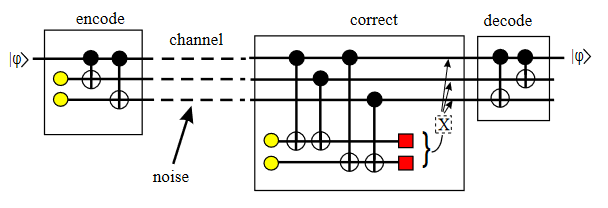
\includegraphics[width=\columnwidth]{figure/3bit.png}
                \caption{3 bit code QEC example}
            \end{figure}
        \end{column}
        \begin{column}{0.5\textwidth}
            \begin{block}{Steps of QEC}
            \begin{enumerate}
                \item encode $\psi$ to 3 bits
                \item sydrome and error detect
                \item error correction and decode
            \end{enumerate}
        \end{block}
        \end{column}
    \end{columns}
    \begin{block}{Toffli Gate}
        Toffili Gate substitute the error detect and error correction.    
    \end{block}
\tiny{Steane. A Tutorial on Quantum Error Correction}
\end{frame}
\begin{frame}
    \frametitle{Surface Code}
    
    However, the experiments was conducted unitl 2012.
\end{frame}
\section{Experiments}
\subsection{3 bit code}
\begin{frame}
    \frametitle{Trapped Ions}
    \begin{columns}
        \begin{column}{0.3\textwidth}
            \centering
            %\includegraphics[width=\columnwidth]{figure/partialEraser1.png}
        \end{column}
        \begin{column}{0.7\textwidth}
            \centering
            %\includegraphics[width=0.8\columnwidth]{figure/partialEraser2.png}
        \end{column}
    \end{columns}
    \begin{block}{Cycle Steps\cite{berut2012experimental}}
        \begin{itemize}
            \item initialize a two wells system. $S_i=k\mathrm{ln(2)}$
            \item lowering the barrier height and apply a tilting force to bring particle into right.
            \item increase the barrier to initial value
        \end{itemize}
    \end{block}
\end{frame}
\begin{frame}
    \frametitle{Trapped Ions}
    \begin{columns}
        \begin{column}{0.28\textwidth}
            \centering
            %\includegraphics[width=\columnwidth]{figure/partialEraser3.png}
        \end{column}
        \begin{column}{0.7\textwidth}
            $r$ is the success rate of erasure, the dissipated heat is
            \[<Q>_{Landauer}=kT(ln(2)+rln(r)+(1-r)ln(1-r))\]

            \begin{block}{Fit function}
                \[<Q>=<Q>_{Landauer}+(Aexp(-t/\tau_k)+1)B/\tau\]
                The thermodynamic limit to information erasure is Landauer bound.
            \end{block}
        \end{column}
    \end{columns}
\end{frame}
\begin{frame}
    \frametitle{Superconduct Qubit}
    \begin{columns}
        \begin{column}{0.5\textwidth}
            \centering
            %\includegraphics[width=\columnwidth]{figure/completeEraser1.png}

            %\includegraphics[width=0.85\columnwidth]{figure/completeEraser2.png}
        \end{column}
        \begin{column}{0.5\textwidth}
            \centering
            \begin{block}{Feedback Operation\cite{jun2014high}}
                \begin{enumerate}
                    \item acquisition of an image of a fluorescent colloidal particle
                    \item determination of particle position from that image using a centroid algorithm
                    \item evaluation of feedback force $F_x=-\partial_xU(x,t)$ at the observed position
                    \item application of electric force with voltage set by electrodes, held constant during the update time $t_s=10\mathrm{ms}$
                \end{enumerate}
            \end{block}

            Erasure protocol and trajectories for full erasure($p=1$) and no erasure($p=0.5$). 
        \end{column}
    \end{columns}
\end{frame}
\subsection{Surface Code}
\begin{frame}
    \frametitle{Surface Code}
    \begin{columns}
        \begin{column}{0.5\textwidth}
            \centering
            %\includegraphics[width=\columnwidth]{figure/completeEraser3.png}
        \end{column}
        \begin{column}{0.5\textwidth}
            The mean work of each cycle is $W(\tau)$
            \[\frac{<W>_\tau}{kT}=\frac{<W>_\infty}{kT}+a\tau^{-1}\] 
            Attention that $frac{<W>_\infty}{kT}=ln2$ for full-erasure and 0 for the noerasure protoncols.
        \end{column}
    \end{columns}
\end{frame}
\begin{frame}
    \frametitle{Surface Code}
    \begin{columns}
        \begin{column}{0.5\textwidth}
            \centering
            %\includegraphics[width=\columnwidth]{figure/magnetic1.png}
        \end{column}
        \begin{column}{0.5\textwidth}
            \centering
            \begin{block}{Experiment Protocol\cite{hong2016experimental}}
                \begin{description}
                    \item[stage1] $H_x$ is applied to saturate the hard axis,removes the energy barrier
                    \item[stage2] $H_y$ is applied along the easy axis to force the magnetization into the 1 state.
                    \item[stage3] $H_x$ is removed to increase the barrier
                    \item[stage4] $H_y$ is removed
                \end{description}
            \end{block}
        \end{column}
    \end{columns}
\end{frame}

\section{Discuss}
\begin{frame}
    \frametitle{Discuss}
    \begin{enumerate}
        \item Landauer limit is repeated using partial erasure and complete erasure.
        \item Landauer limit is general in at least two different materials.
    \end{enumerate}
\end{frame}
\section{Reference}
\begin{frame}[allowframebreaks]
    \frametitle{Reference}
    \printbibliography
\end{frame}
\begin{frame}
    \centering{THANKS!}
\end{frame}
\end{document}